\documentclass{article}
\usepackage{graphicx,caption}
\usepackage{enumitem}
\usepackage{epstopdf,subcaption}
\usepackage{psfrag}
\usepackage{amsmath,amssymb,epsf}
\usepackage{verbatim}
\usepackage[hyphens]{url}
\usepackage{amsmath}
\usepackage{color}
\usepackage{bbm}
\usepackage{listings}
\usepackage{setspace}
\usepackage{float}
\definecolor{Code}{rgb}{0,0,0}
\definecolor{Decorators}{rgb}{0.5,0.5,0.5}
\definecolor{Numbers}{rgb}{0.5,0,0}
\definecolor{MatchingBrackets}{rgb}{0.25,0.5,0.5}
\definecolor{Keywords}{rgb}{0,0,1}
\definecolor{self}{rgb}{0,0,0}
\definecolor{Strings}{rgb}{0,0.63,0}
\definecolor{Comments}{rgb}{0,0.63,1}
\definecolor{Backquotes}{rgb}{0,0,0}
\definecolor{Classname}{rgb}{0,0,0}
\definecolor{FunctionName}{rgb}{0,0,0}
\definecolor{Operators}{rgb}{0,0,0}
\definecolor{Background}{rgb}{0.98,0.98,0.98}
\lstdefinelanguage{Python}{
	numbers=left,
	numberstyle=\footnotesize,
	numbersep=1em,
	xleftmargin=1em,
	framextopmargin=2em,
	framexbottommargin=2em,
	showspaces=false,
	showtabs=false,
	showstringspaces=false,
	frame=l,
	tabsize=4,
	% Basic
	basicstyle=\ttfamily\footnotesize\setstretch{1},
	backgroundcolor=\color{Background},
	% Comments
	commentstyle=\color{Comments}\slshape,
	% Strings
	stringstyle=\color{Strings},
	morecomment=[s][\color{Strings}]{"""}{"""},
	morecomment=[s][\color{Strings}]{'''}{'''},
	% keywords
	morekeywords={import,from,class,def,for,while,if,is,in,elif,else,not,and,or
		,print,break,continue,return,True,False,None,access,as,,del,except,exec
		,finally,global,import,lambda,pass,print,raise,try,assert},
	keywordstyle={\color{Keywords}\bfseries},
	% additional keywords
	morekeywords={[2]@invariant},
	keywordstyle={[2]\color{Decorators}\slshape},
	emph={self},
	emphstyle={\color{self}\slshape},
	%
}

%%% Change the following flag to toggle between questions or solutions
\def\solutions{1}

\pagestyle{empty} \addtolength{\textwidth}{1.0in}
\addtolength{\textheight}{0.5in}
\addtolength{\oddsidemargin}{-0.5in}
\addtolength{\evensidemargin}{-0.5in}
\newcommand{\ruleskip}{\bigskip\hrule\bigskip}
\newcommand{\nodify}[1]{{\sc #1}}
\newcommand{\points}[1]{{\textbf{[#1 points]}}}
\newcommand{\subquestionpoints}[1]{{[#1 points]}}
\newenvironment{answer}{{\bf Answer:} \sf \begingroup\color{red}}{\endgroup}%

\newcommand{\bitem}{\begin{list}{$\bullet$}%
		{\setlength{\itemsep}{0pt}\setlength{\topsep}{0pt}%
			\setlength{\rightmargin}{0pt}}}
	\newcommand{\eitem}{\end{list}}

\setlength{\parindent}{0pt} \setlength{\parskip}{0.5ex}
\setlength{\unitlength}{1cm}

\renewcommand{\Re}{{\mathbb R}}
\newcommand{\R}{\mathbb{R}}
\newcommand{\what}[1]{\widehat{#1}}

\renewcommand{\comment}[1]{}
\newcommand{\mc}[1]{\mathcal{#1}}
\newcommand{\half}{\frac{1}{2}}

\begin{document}
	
	\pagestyle{myheadings} \markboth{}{CS229 Problem Set \#2}
	
	\ifnum\solutions=1 {
		{\huge\noindent CS 229, Fall 2018\\
			Problem Set \#2 Solutions: Supervised Learning II}\\\\
		YOUR NAME HERE (\texttt{YOUR SUNET HERE})
	} \else {\huge
		\noindent CS 229, Fall 2018\\
		Problem Set \#2: Supervised Learning II
	} \fi
	
	\ruleskip
	
	{\bf Due Wednesday, Oct 31 at 11:59 pm on Gradescope.}
	
	\medskip
	
	\clearpage
\item \points{15} {\bf Logistic Regression: Training stability}

In this problem, we will be delving deeper into the workings of logistic
regression. The goal of this problem is to help you develop your skills
debugging machine learning algorithms (which can be very different from
debugging software in general).

We have provided a implementation of logistic regression in
\texttt{src/p01\_lr.py}, and two labeled datasets $A$ and $B$ in
\texttt{data/ds1\_a.txt} and \texttt{data/ds1\_b.txt}

Please do not modify the code for the logistic regression training algorithm
for this problem. First, run the given logistic regression code to train two
different models on $A$ and $B$. You can run the code by simply executing 
\texttt{python p01\_lr.py} in the \texttt{src} directory.

\begin{enumerate}

  \item \subquestionpoints{2}
What is the most notable difference in training the logistic regression model
on datasets $A$ and $B$?

\ifnum\solutions=1 {
  \begin{answer}
    Training on dataset A finished with few iterations, while with B it seems like a dead loop.
    
    P.S. I think the line \texttt{probs = 1. / (1 + np.exp(margins))} in the \texttt{cal\_grad} function of \texttt{src/p01\_lr.py} cannot be seen as probability (of a conventional Bernoulli distribution) because it is just a metric of margin.
    
    In fact if we choose $ \{0,1\} $ to represent label, we can write down the binary Bernoulli distribution $ B(\phi) $ and using GLM method to computer the expression of $ \phi $ as $ \frac{1}{1+\exp{-\theta^Tx}} $ so that this can be regarded as probability of being 1 given sample x.
    
    But that line only measure the margin between the point and the decision boundary. It cannot represent the probability of a point being classified as positive. 
    
\end{answer}

} \fi


  \item \subquestionpoints{5}
Investigate why the training procedure behaves unexpectedly on dataset $B$, but
not on $A$. Provide hard evidence (in the form of math, code, plots, etc.) to
corroborate your hypothesis for the misbehavior. Remember, you should address
why your explanation does \emph{not} apply to $A$.

\textbf{Hint}: The issue is not a numerical rounding or over/underflow error.

\ifnum\solutions=1 {
  
\begin{answer}

\begin{figure}[htbp]
\begin{subfigure}[b]{0.5\linewidth}
    \centering
    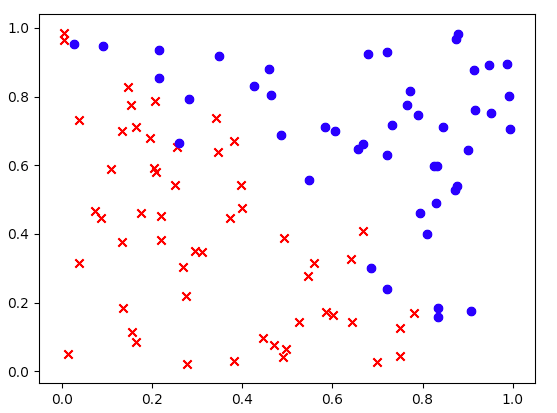
\includegraphics[width=\linewidth]{pics/F1b-b.png}
    \caption{Dataset A}\label{fig:dataset-a}
\end{subfigure}
\begin{subfigure}[b]{0.5\linewidth}
    \centering
    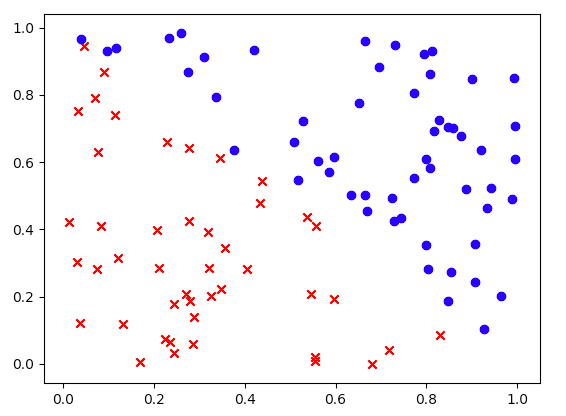
\includegraphics[width=\linewidth]{pics/F1b-a.png}
    \caption{Dataset B}\label{fig:dataset-b}
\end{subfigure}
\caption{Datasets}
\label{fig:datasets}
\end{figure}

Figure~\subref{fig:dataset-a} and Figure~\subref{fig:dataset-b} shows the two datasets. The problem is that dataset B is perfectly linearly separable. 

Consider optimizing objective:

$$
    L(\theta) = \prod_{i=1}^mp(y^{(i)}|x^{(i)};\theta) = \frac{1}{1 + e^{-y^{(i)}\theta^T x^{(i)}}}
$$

    Since the algorithm tries to find the maximum likelihood. if the data is linearly separable(i.e. all $y^{(i)}\theta^T x^{(i)}$ can be positive), every $ \frac{1}{1 + e^{-y^{(i)}\theta^T x^{(i)}}} $ can be small by augmenting the norm of $ \theta $ so after perfectly separate them the algorithm tends to augment $ \theta $ to infinity.
    
    If the data isn't linearly separable(i.e.  $\exists\  y^{(i)}\theta^T x^{(i)}$ to be negative), in this case, the algorithm cannot augment $ \theta $ infinitely since the negative $y^{(i)}\theta^T x^{(i)}$ constraints $ \frac{1}{1 + e^{-y^{(i)}\theta^T x^{(i)}}} $  to be very small while $ \|\theta\| $ is large. just like the regularization term. So there is a trade-off while maximizing the likelihood. 
\end{answer}


} \fi


  \item \subquestionpoints{5}
For each of these possible modifications, state whether or not it would lead to
the provided training algorithm converging on datasets such as $B$. Justify your
answers.
\begin{enumerate}
  \item Using a different constant learning rate.
  \item Decreasing the learning rate over time (e.g. scaling the initial
  learning rate by $1/t^2$, where $t$ is the number of gradient descent
  iterations thus far).
  \item Linear scaling of the input features.
  \item Adding a regularization term $\|\theta\|_2^2$ to the loss function.
  \item Adding zero-mean Gaussian noise to the training data or labels.
\end{enumerate}
 
\ifnum\solutions=1 {
  \begin{answer}
\begin{enumerate}
    \item No. $L(\theta)$ can still be arbitrarily large.
  \item Yes. When the learning rate is sufficiently small, the update to $\theta$ will be small, and it will be judged to be converged by the algorithm.
  \item No. The dataset will still be linearly seperable.
  \item Yes. In this case, scaling $\theta$ will not make the objective arbitrarily large.
  \item Yes. This will very likely make the dataset not linearly seperable.
  \item Yes. This will make the dataset not linearly separable, and easier to approach the global minimum.
\end{enumerate}

\end{answer}

} \fi

 
  
  \item \subquestionpoints{2}
Support vector machines (SVMs) are an alternative machine learning model that we discussed in class.
We have provided you an SVM implementation (using a radial basis function (RBF) kernel) within \texttt{src/svm.py} (You should not need to modify that code).

One important part of training an SVM parameterized by an RBF kernel is choosing an appropriate kernel radius.

Complete the \texttt{compute\_best\_svm\_radius} by writing code to compute the best SVM radius which maximizes accuracy on the validation dataset.

The provided code will use your \texttt{compute\_best\_svm\_radius} to compute and then write the best radius into \texttt{output/p06\_optimal\_radius}.

\ifnum\solutions=1 {
  \begin{answer}
    0.1 works best. The accuracy is 0.9695340501792115.
\end{answer}

} \fi



\end{enumerate}

\textbf{Hint:} Recall the distinction between functional margin and geometric
margin.

	
	\begin{enumerate}[wide, labelwidth=!, labelindent=0pt]
		
		\clearpage
\item \points{15} {\bf Logistic Regression: Training stability}

In this problem, we will be delving deeper into the workings of logistic
regression. The goal of this problem is to help you develop your skills
debugging machine learning algorithms (which can be very different from
debugging software in general).

We have provided a implementation of logistic regression in
\texttt{src/p01\_lr.py}, and two labeled datasets $A$ and $B$ in
\texttt{data/ds1\_a.txt} and \texttt{data/ds1\_b.txt}

Please do not modify the code for the logistic regression training algorithm
for this problem. First, run the given logistic regression code to train two
different models on $A$ and $B$. You can run the code by simply executing 
\texttt{python p01\_lr.py} in the \texttt{src} directory.

\begin{enumerate}

  \item \subquestionpoints{2}
What is the most notable difference in training the logistic regression model
on datasets $A$ and $B$?

\ifnum\solutions=1 {
  \begin{answer}
    Training on dataset A finished with few iterations, while with B it seems like a dead loop.
    
    P.S. I think the line \texttt{probs = 1. / (1 + np.exp(margins))} in the \texttt{cal\_grad} function of \texttt{src/p01\_lr.py} cannot be seen as probability (of a conventional Bernoulli distribution) because it is just a metric of margin.
    
    In fact if we choose $ \{0,1\} $ to represent label, we can write down the binary Bernoulli distribution $ B(\phi) $ and using GLM method to computer the expression of $ \phi $ as $ \frac{1}{1+\exp{-\theta^Tx}} $ so that this can be regarded as probability of being 1 given sample x.
    
    But that line only measure the margin between the point and the decision boundary. It cannot represent the probability of a point being classified as positive. 
    
\end{answer}

} \fi


  \item \subquestionpoints{5}
Investigate why the training procedure behaves unexpectedly on dataset $B$, but
not on $A$. Provide hard evidence (in the form of math, code, plots, etc.) to
corroborate your hypothesis for the misbehavior. Remember, you should address
why your explanation does \emph{not} apply to $A$.

\textbf{Hint}: The issue is not a numerical rounding or over/underflow error.

\ifnum\solutions=1 {
  
\begin{answer}

\begin{figure}[htbp]
\begin{subfigure}[b]{0.5\linewidth}
    \centering
    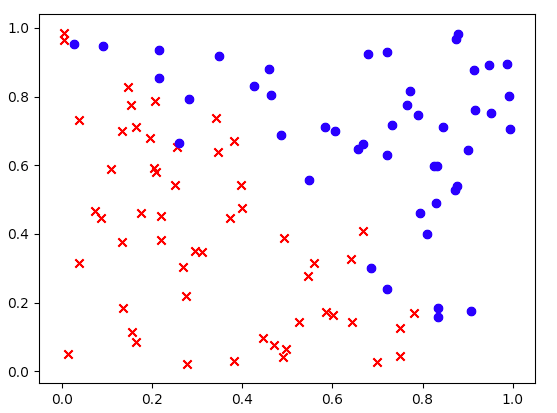
\includegraphics[width=\linewidth]{pics/F1b-b.png}
    \caption{Dataset A}\label{fig:dataset-a}
\end{subfigure}
\begin{subfigure}[b]{0.5\linewidth}
    \centering
    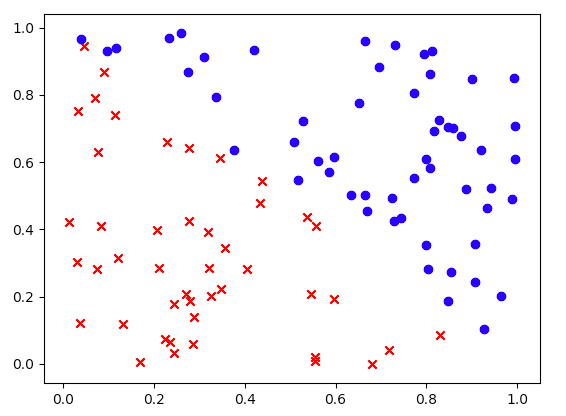
\includegraphics[width=\linewidth]{pics/F1b-a.png}
    \caption{Dataset B}\label{fig:dataset-b}
\end{subfigure}
\caption{Datasets}
\label{fig:datasets}
\end{figure}

Figure~\subref{fig:dataset-a} and Figure~\subref{fig:dataset-b} shows the two datasets. The problem is that dataset B is perfectly linearly separable. 

Consider optimizing objective:

$$
    L(\theta) = \prod_{i=1}^mp(y^{(i)}|x^{(i)};\theta) = \frac{1}{1 + e^{-y^{(i)}\theta^T x^{(i)}}}
$$

    Since the algorithm tries to find the maximum likelihood. if the data is linearly separable(i.e. all $y^{(i)}\theta^T x^{(i)}$ can be positive), every $ \frac{1}{1 + e^{-y^{(i)}\theta^T x^{(i)}}} $ can be small by augmenting the norm of $ \theta $ so after perfectly separate them the algorithm tends to augment $ \theta $ to infinity.
    
    If the data isn't linearly separable(i.e.  $\exists\  y^{(i)}\theta^T x^{(i)}$ to be negative), in this case, the algorithm cannot augment $ \theta $ infinitely since the negative $y^{(i)}\theta^T x^{(i)}$ constraints $ \frac{1}{1 + e^{-y^{(i)}\theta^T x^{(i)}}} $  to be very small while $ \|\theta\| $ is large. just like the regularization term. So there is a trade-off while maximizing the likelihood. 
\end{answer}


} \fi


  \item \subquestionpoints{5}
For each of these possible modifications, state whether or not it would lead to
the provided training algorithm converging on datasets such as $B$. Justify your
answers.
\begin{enumerate}
  \item Using a different constant learning rate.
  \item Decreasing the learning rate over time (e.g. scaling the initial
  learning rate by $1/t^2$, where $t$ is the number of gradient descent
  iterations thus far).
  \item Linear scaling of the input features.
  \item Adding a regularization term $\|\theta\|_2^2$ to the loss function.
  \item Adding zero-mean Gaussian noise to the training data or labels.
\end{enumerate}
 
\ifnum\solutions=1 {
  \begin{answer}
\begin{enumerate}
    \item No. $L(\theta)$ can still be arbitrarily large.
  \item Yes. When the learning rate is sufficiently small, the update to $\theta$ will be small, and it will be judged to be converged by the algorithm.
  \item No. The dataset will still be linearly seperable.
  \item Yes. In this case, scaling $\theta$ will not make the objective arbitrarily large.
  \item Yes. This will very likely make the dataset not linearly seperable.
  \item Yes. This will make the dataset not linearly separable, and easier to approach the global minimum.
\end{enumerate}

\end{answer}

} \fi

 
  
  \item \subquestionpoints{2}
Support vector machines (SVMs) are an alternative machine learning model that we discussed in class.
We have provided you an SVM implementation (using a radial basis function (RBF) kernel) within \texttt{src/svm.py} (You should not need to modify that code).

One important part of training an SVM parameterized by an RBF kernel is choosing an appropriate kernel radius.

Complete the \texttt{compute\_best\_svm\_radius} by writing code to compute the best SVM radius which maximizes accuracy on the validation dataset.

The provided code will use your \texttt{compute\_best\_svm\_radius} to compute and then write the best radius into \texttt{output/p06\_optimal\_radius}.

\ifnum\solutions=1 {
  \begin{answer}
    0.1 works best. The accuracy is 0.9695340501792115.
\end{answer}

} \fi



\end{enumerate}

\textbf{Hint:} Recall the distinction between functional margin and geometric
margin.

		
		\clearpage
\item \points{15} {\bf Logistic Regression: Training stability}

In this problem, we will be delving deeper into the workings of logistic
regression. The goal of this problem is to help you develop your skills
debugging machine learning algorithms (which can be very different from
debugging software in general).

We have provided a implementation of logistic regression in
\texttt{src/p01\_lr.py}, and two labeled datasets $A$ and $B$ in
\texttt{data/ds1\_a.txt} and \texttt{data/ds1\_b.txt}

Please do not modify the code for the logistic regression training algorithm
for this problem. First, run the given logistic regression code to train two
different models on $A$ and $B$. You can run the code by simply executing 
\texttt{python p01\_lr.py} in the \texttt{src} directory.

\begin{enumerate}

  \item \subquestionpoints{2}
What is the most notable difference in training the logistic regression model
on datasets $A$ and $B$?

\ifnum\solutions=1 {
  \begin{answer}
    Training on dataset A finished with few iterations, while with B it seems like a dead loop.
    
    P.S. I think the line \texttt{probs = 1. / (1 + np.exp(margins))} in the \texttt{cal\_grad} function of \texttt{src/p01\_lr.py} cannot be seen as probability (of a conventional Bernoulli distribution) because it is just a metric of margin.
    
    In fact if we choose $ \{0,1\} $ to represent label, we can write down the binary Bernoulli distribution $ B(\phi) $ and using GLM method to computer the expression of $ \phi $ as $ \frac{1}{1+\exp{-\theta^Tx}} $ so that this can be regarded as probability of being 1 given sample x.
    
    But that line only measure the margin between the point and the decision boundary. It cannot represent the probability of a point being classified as positive. 
    
\end{answer}

} \fi


  \item \subquestionpoints{5}
Investigate why the training procedure behaves unexpectedly on dataset $B$, but
not on $A$. Provide hard evidence (in the form of math, code, plots, etc.) to
corroborate your hypothesis for the misbehavior. Remember, you should address
why your explanation does \emph{not} apply to $A$.

\textbf{Hint}: The issue is not a numerical rounding or over/underflow error.

\ifnum\solutions=1 {
  
\begin{answer}

\begin{figure}[htbp]
\begin{subfigure}[b]{0.5\linewidth}
    \centering
    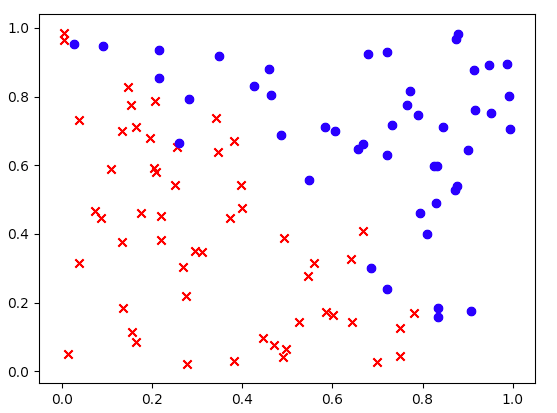
\includegraphics[width=\linewidth]{pics/F1b-b.png}
    \caption{Dataset A}\label{fig:dataset-a}
\end{subfigure}
\begin{subfigure}[b]{0.5\linewidth}
    \centering
    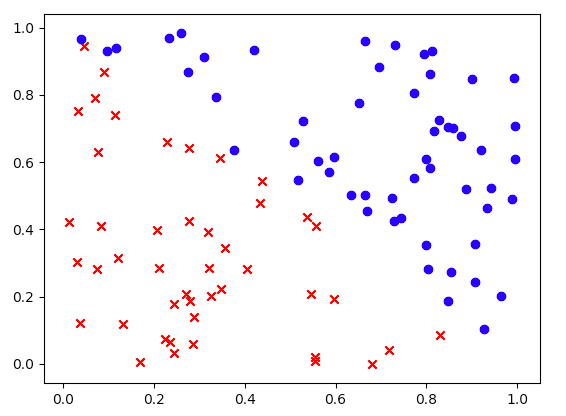
\includegraphics[width=\linewidth]{pics/F1b-a.png}
    \caption{Dataset B}\label{fig:dataset-b}
\end{subfigure}
\caption{Datasets}
\label{fig:datasets}
\end{figure}

Figure~\subref{fig:dataset-a} and Figure~\subref{fig:dataset-b} shows the two datasets. The problem is that dataset B is perfectly linearly separable. 

Consider optimizing objective:

$$
    L(\theta) = \prod_{i=1}^mp(y^{(i)}|x^{(i)};\theta) = \frac{1}{1 + e^{-y^{(i)}\theta^T x^{(i)}}}
$$

    Since the algorithm tries to find the maximum likelihood. if the data is linearly separable(i.e. all $y^{(i)}\theta^T x^{(i)}$ can be positive), every $ \frac{1}{1 + e^{-y^{(i)}\theta^T x^{(i)}}} $ can be small by augmenting the norm of $ \theta $ so after perfectly separate them the algorithm tends to augment $ \theta $ to infinity.
    
    If the data isn't linearly separable(i.e.  $\exists\  y^{(i)}\theta^T x^{(i)}$ to be negative), in this case, the algorithm cannot augment $ \theta $ infinitely since the negative $y^{(i)}\theta^T x^{(i)}$ constraints $ \frac{1}{1 + e^{-y^{(i)}\theta^T x^{(i)}}} $  to be very small while $ \|\theta\| $ is large. just like the regularization term. So there is a trade-off while maximizing the likelihood. 
\end{answer}


} \fi


  \item \subquestionpoints{5}
For each of these possible modifications, state whether or not it would lead to
the provided training algorithm converging on datasets such as $B$. Justify your
answers.
\begin{enumerate}
  \item Using a different constant learning rate.
  \item Decreasing the learning rate over time (e.g. scaling the initial
  learning rate by $1/t^2$, where $t$ is the number of gradient descent
  iterations thus far).
  \item Linear scaling of the input features.
  \item Adding a regularization term $\|\theta\|_2^2$ to the loss function.
  \item Adding zero-mean Gaussian noise to the training data or labels.
\end{enumerate}
 
\ifnum\solutions=1 {
  \begin{answer}
\begin{enumerate}
    \item No. $L(\theta)$ can still be arbitrarily large.
  \item Yes. When the learning rate is sufficiently small, the update to $\theta$ will be small, and it will be judged to be converged by the algorithm.
  \item No. The dataset will still be linearly seperable.
  \item Yes. In this case, scaling $\theta$ will not make the objective arbitrarily large.
  \item Yes. This will very likely make the dataset not linearly seperable.
  \item Yes. This will make the dataset not linearly separable, and easier to approach the global minimum.
\end{enumerate}

\end{answer}

} \fi

 
  
  \item \subquestionpoints{2}
Support vector machines (SVMs) are an alternative machine learning model that we discussed in class.
We have provided you an SVM implementation (using a radial basis function (RBF) kernel) within \texttt{src/svm.py} (You should not need to modify that code).

One important part of training an SVM parameterized by an RBF kernel is choosing an appropriate kernel radius.

Complete the \texttt{compute\_best\_svm\_radius} by writing code to compute the best SVM radius which maximizes accuracy on the validation dataset.

The provided code will use your \texttt{compute\_best\_svm\_radius} to compute and then write the best radius into \texttt{output/p06\_optimal\_radius}.

\ifnum\solutions=1 {
  \begin{answer}
    0.1 works best. The accuracy is 0.9695340501792115.
\end{answer}

} \fi



\end{enumerate}

\textbf{Hint:} Recall the distinction between functional margin and geometric
margin.

		
		\clearpage
\item \points{15} {\bf Logistic Regression: Training stability}

In this problem, we will be delving deeper into the workings of logistic
regression. The goal of this problem is to help you develop your skills
debugging machine learning algorithms (which can be very different from
debugging software in general).

We have provided a implementation of logistic regression in
\texttt{src/p01\_lr.py}, and two labeled datasets $A$ and $B$ in
\texttt{data/ds1\_a.txt} and \texttt{data/ds1\_b.txt}

Please do not modify the code for the logistic regression training algorithm
for this problem. First, run the given logistic regression code to train two
different models on $A$ and $B$. You can run the code by simply executing 
\texttt{python p01\_lr.py} in the \texttt{src} directory.

\begin{enumerate}

  \item \subquestionpoints{2}
What is the most notable difference in training the logistic regression model
on datasets $A$ and $B$?

\ifnum\solutions=1 {
  \begin{answer}
    Training on dataset A finished with few iterations, while with B it seems like a dead loop.
    
    P.S. I think the line \texttt{probs = 1. / (1 + np.exp(margins))} in the \texttt{cal\_grad} function of \texttt{src/p01\_lr.py} cannot be seen as probability (of a conventional Bernoulli distribution) because it is just a metric of margin.
    
    In fact if we choose $ \{0,1\} $ to represent label, we can write down the binary Bernoulli distribution $ B(\phi) $ and using GLM method to computer the expression of $ \phi $ as $ \frac{1}{1+\exp{-\theta^Tx}} $ so that this can be regarded as probability of being 1 given sample x.
    
    But that line only measure the margin between the point and the decision boundary. It cannot represent the probability of a point being classified as positive. 
    
\end{answer}

} \fi


  \item \subquestionpoints{5}
Investigate why the training procedure behaves unexpectedly on dataset $B$, but
not on $A$. Provide hard evidence (in the form of math, code, plots, etc.) to
corroborate your hypothesis for the misbehavior. Remember, you should address
why your explanation does \emph{not} apply to $A$.

\textbf{Hint}: The issue is not a numerical rounding or over/underflow error.

\ifnum\solutions=1 {
  
\begin{answer}

\begin{figure}[htbp]
\begin{subfigure}[b]{0.5\linewidth}
    \centering
    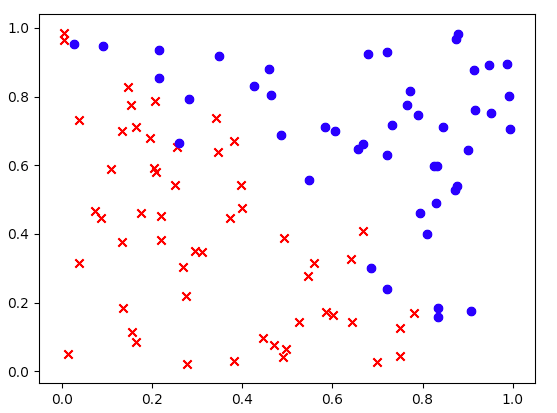
\includegraphics[width=\linewidth]{pics/F1b-b.png}
    \caption{Dataset A}\label{fig:dataset-a}
\end{subfigure}
\begin{subfigure}[b]{0.5\linewidth}
    \centering
    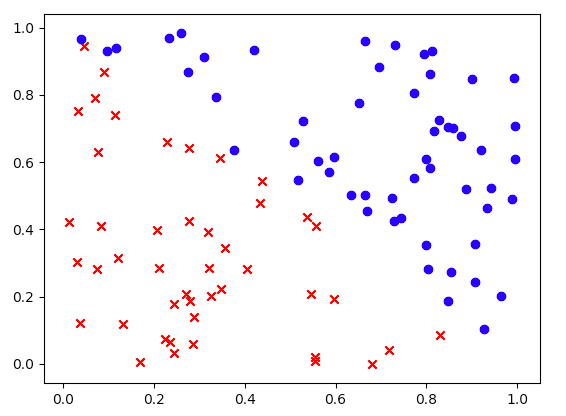
\includegraphics[width=\linewidth]{pics/F1b-a.png}
    \caption{Dataset B}\label{fig:dataset-b}
\end{subfigure}
\caption{Datasets}
\label{fig:datasets}
\end{figure}

Figure~\subref{fig:dataset-a} and Figure~\subref{fig:dataset-b} shows the two datasets. The problem is that dataset B is perfectly linearly separable. 

Consider optimizing objective:

$$
    L(\theta) = \prod_{i=1}^mp(y^{(i)}|x^{(i)};\theta) = \frac{1}{1 + e^{-y^{(i)}\theta^T x^{(i)}}}
$$

    Since the algorithm tries to find the maximum likelihood. if the data is linearly separable(i.e. all $y^{(i)}\theta^T x^{(i)}$ can be positive), every $ \frac{1}{1 + e^{-y^{(i)}\theta^T x^{(i)}}} $ can be small by augmenting the norm of $ \theta $ so after perfectly separate them the algorithm tends to augment $ \theta $ to infinity.
    
    If the data isn't linearly separable(i.e.  $\exists\  y^{(i)}\theta^T x^{(i)}$ to be negative), in this case, the algorithm cannot augment $ \theta $ infinitely since the negative $y^{(i)}\theta^T x^{(i)}$ constraints $ \frac{1}{1 + e^{-y^{(i)}\theta^T x^{(i)}}} $  to be very small while $ \|\theta\| $ is large. just like the regularization term. So there is a trade-off while maximizing the likelihood. 
\end{answer}


} \fi


  \item \subquestionpoints{5}
For each of these possible modifications, state whether or not it would lead to
the provided training algorithm converging on datasets such as $B$. Justify your
answers.
\begin{enumerate}
  \item Using a different constant learning rate.
  \item Decreasing the learning rate over time (e.g. scaling the initial
  learning rate by $1/t^2$, where $t$ is the number of gradient descent
  iterations thus far).
  \item Linear scaling of the input features.
  \item Adding a regularization term $\|\theta\|_2^2$ to the loss function.
  \item Adding zero-mean Gaussian noise to the training data or labels.
\end{enumerate}
 
\ifnum\solutions=1 {
  \begin{answer}
\begin{enumerate}
    \item No. $L(\theta)$ can still be arbitrarily large.
  \item Yes. When the learning rate is sufficiently small, the update to $\theta$ will be small, and it will be judged to be converged by the algorithm.
  \item No. The dataset will still be linearly seperable.
  \item Yes. In this case, scaling $\theta$ will not make the objective arbitrarily large.
  \item Yes. This will very likely make the dataset not linearly seperable.
  \item Yes. This will make the dataset not linearly separable, and easier to approach the global minimum.
\end{enumerate}

\end{answer}

} \fi

 
  
  \item \subquestionpoints{2}
Support vector machines (SVMs) are an alternative machine learning model that we discussed in class.
We have provided you an SVM implementation (using a radial basis function (RBF) kernel) within \texttt{src/svm.py} (You should not need to modify that code).

One important part of training an SVM parameterized by an RBF kernel is choosing an appropriate kernel radius.

Complete the \texttt{compute\_best\_svm\_radius} by writing code to compute the best SVM radius which maximizes accuracy on the validation dataset.

The provided code will use your \texttt{compute\_best\_svm\_radius} to compute and then write the best radius into \texttt{output/p06\_optimal\_radius}.

\ifnum\solutions=1 {
  \begin{answer}
    0.1 works best. The accuracy is 0.9695340501792115.
\end{answer}

} \fi



\end{enumerate}

\textbf{Hint:} Recall the distinction between functional margin and geometric
margin.

		
		\clearpage
\item \points{15} {\bf Logistic Regression: Training stability}

In this problem, we will be delving deeper into the workings of logistic
regression. The goal of this problem is to help you develop your skills
debugging machine learning algorithms (which can be very different from
debugging software in general).

We have provided a implementation of logistic regression in
\texttt{src/p01\_lr.py}, and two labeled datasets $A$ and $B$ in
\texttt{data/ds1\_a.txt} and \texttt{data/ds1\_b.txt}

Please do not modify the code for the logistic regression training algorithm
for this problem. First, run the given logistic regression code to train two
different models on $A$ and $B$. You can run the code by simply executing 
\texttt{python p01\_lr.py} in the \texttt{src} directory.

\begin{enumerate}

  \item \subquestionpoints{2}
What is the most notable difference in training the logistic regression model
on datasets $A$ and $B$?

\ifnum\solutions=1 {
  \begin{answer}
    Training on dataset A finished with few iterations, while with B it seems like a dead loop.
    
    P.S. I think the line \texttt{probs = 1. / (1 + np.exp(margins))} in the \texttt{cal\_grad} function of \texttt{src/p01\_lr.py} cannot be seen as probability (of a conventional Bernoulli distribution) because it is just a metric of margin.
    
    In fact if we choose $ \{0,1\} $ to represent label, we can write down the binary Bernoulli distribution $ B(\phi) $ and using GLM method to computer the expression of $ \phi $ as $ \frac{1}{1+\exp{-\theta^Tx}} $ so that this can be regarded as probability of being 1 given sample x.
    
    But that line only measure the margin between the point and the decision boundary. It cannot represent the probability of a point being classified as positive. 
    
\end{answer}

} \fi


  \item \subquestionpoints{5}
Investigate why the training procedure behaves unexpectedly on dataset $B$, but
not on $A$. Provide hard evidence (in the form of math, code, plots, etc.) to
corroborate your hypothesis for the misbehavior. Remember, you should address
why your explanation does \emph{not} apply to $A$.

\textbf{Hint}: The issue is not a numerical rounding or over/underflow error.

\ifnum\solutions=1 {
  
\begin{answer}

\begin{figure}[htbp]
\begin{subfigure}[b]{0.5\linewidth}
    \centering
    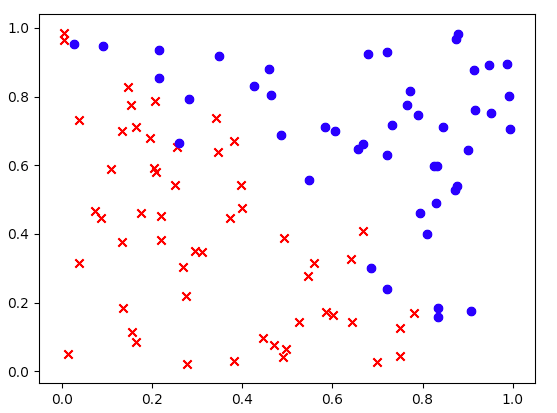
\includegraphics[width=\linewidth]{pics/F1b-b.png}
    \caption{Dataset A}\label{fig:dataset-a}
\end{subfigure}
\begin{subfigure}[b]{0.5\linewidth}
    \centering
    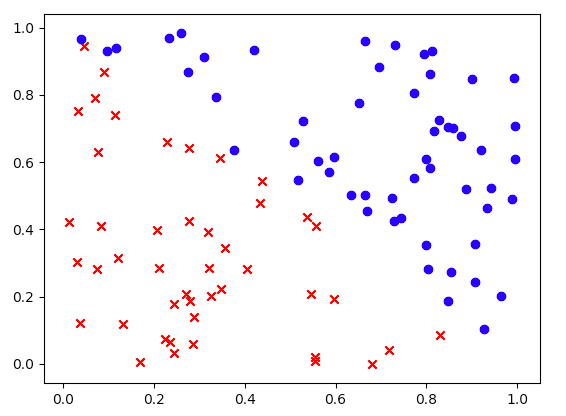
\includegraphics[width=\linewidth]{pics/F1b-a.png}
    \caption{Dataset B}\label{fig:dataset-b}
\end{subfigure}
\caption{Datasets}
\label{fig:datasets}
\end{figure}

Figure~\subref{fig:dataset-a} and Figure~\subref{fig:dataset-b} shows the two datasets. The problem is that dataset B is perfectly linearly separable. 

Consider optimizing objective:

$$
    L(\theta) = \prod_{i=1}^mp(y^{(i)}|x^{(i)};\theta) = \frac{1}{1 + e^{-y^{(i)}\theta^T x^{(i)}}}
$$

    Since the algorithm tries to find the maximum likelihood. if the data is linearly separable(i.e. all $y^{(i)}\theta^T x^{(i)}$ can be positive), every $ \frac{1}{1 + e^{-y^{(i)}\theta^T x^{(i)}}} $ can be small by augmenting the norm of $ \theta $ so after perfectly separate them the algorithm tends to augment $ \theta $ to infinity.
    
    If the data isn't linearly separable(i.e.  $\exists\  y^{(i)}\theta^T x^{(i)}$ to be negative), in this case, the algorithm cannot augment $ \theta $ infinitely since the negative $y^{(i)}\theta^T x^{(i)}$ constraints $ \frac{1}{1 + e^{-y^{(i)}\theta^T x^{(i)}}} $  to be very small while $ \|\theta\| $ is large. just like the regularization term. So there is a trade-off while maximizing the likelihood. 
\end{answer}


} \fi


  \item \subquestionpoints{5}
For each of these possible modifications, state whether or not it would lead to
the provided training algorithm converging on datasets such as $B$. Justify your
answers.
\begin{enumerate}
  \item Using a different constant learning rate.
  \item Decreasing the learning rate over time (e.g. scaling the initial
  learning rate by $1/t^2$, where $t$ is the number of gradient descent
  iterations thus far).
  \item Linear scaling of the input features.
  \item Adding a regularization term $\|\theta\|_2^2$ to the loss function.
  \item Adding zero-mean Gaussian noise to the training data or labels.
\end{enumerate}
 
\ifnum\solutions=1 {
  \begin{answer}
\begin{enumerate}
    \item No. $L(\theta)$ can still be arbitrarily large.
  \item Yes. When the learning rate is sufficiently small, the update to $\theta$ will be small, and it will be judged to be converged by the algorithm.
  \item No. The dataset will still be linearly seperable.
  \item Yes. In this case, scaling $\theta$ will not make the objective arbitrarily large.
  \item Yes. This will very likely make the dataset not linearly seperable.
  \item Yes. This will make the dataset not linearly separable, and easier to approach the global minimum.
\end{enumerate}

\end{answer}

} \fi

 
  
  \item \subquestionpoints{2}
Support vector machines (SVMs) are an alternative machine learning model that we discussed in class.
We have provided you an SVM implementation (using a radial basis function (RBF) kernel) within \texttt{src/svm.py} (You should not need to modify that code).

One important part of training an SVM parameterized by an RBF kernel is choosing an appropriate kernel radius.

Complete the \texttt{compute\_best\_svm\_radius} by writing code to compute the best SVM radius which maximizes accuracy on the validation dataset.

The provided code will use your \texttt{compute\_best\_svm\_radius} to compute and then write the best radius into \texttt{output/p06\_optimal\_radius}.

\ifnum\solutions=1 {
  \begin{answer}
    0.1 works best. The accuracy is 0.9695340501792115.
\end{answer}

} \fi



\end{enumerate}

\textbf{Hint:} Recall the distinction between functional margin and geometric
margin.

		
		\clearpage
\item \points{15} {\bf Logistic Regression: Training stability}

In this problem, we will be delving deeper into the workings of logistic
regression. The goal of this problem is to help you develop your skills
debugging machine learning algorithms (which can be very different from
debugging software in general).

We have provided a implementation of logistic regression in
\texttt{src/p01\_lr.py}, and two labeled datasets $A$ and $B$ in
\texttt{data/ds1\_a.txt} and \texttt{data/ds1\_b.txt}

Please do not modify the code for the logistic regression training algorithm
for this problem. First, run the given logistic regression code to train two
different models on $A$ and $B$. You can run the code by simply executing 
\texttt{python p01\_lr.py} in the \texttt{src} directory.

\begin{enumerate}

  \item \subquestionpoints{2}
What is the most notable difference in training the logistic regression model
on datasets $A$ and $B$?

\ifnum\solutions=1 {
  \begin{answer}
    Training on dataset A finished with few iterations, while with B it seems like a dead loop.
    
    P.S. I think the line \texttt{probs = 1. / (1 + np.exp(margins))} in the \texttt{cal\_grad} function of \texttt{src/p01\_lr.py} cannot be seen as probability (of a conventional Bernoulli distribution) because it is just a metric of margin.
    
    In fact if we choose $ \{0,1\} $ to represent label, we can write down the binary Bernoulli distribution $ B(\phi) $ and using GLM method to computer the expression of $ \phi $ as $ \frac{1}{1+\exp{-\theta^Tx}} $ so that this can be regarded as probability of being 1 given sample x.
    
    But that line only measure the margin between the point and the decision boundary. It cannot represent the probability of a point being classified as positive. 
    
\end{answer}

} \fi


  \item \subquestionpoints{5}
Investigate why the training procedure behaves unexpectedly on dataset $B$, but
not on $A$. Provide hard evidence (in the form of math, code, plots, etc.) to
corroborate your hypothesis for the misbehavior. Remember, you should address
why your explanation does \emph{not} apply to $A$.

\textbf{Hint}: The issue is not a numerical rounding or over/underflow error.

\ifnum\solutions=1 {
  
\begin{answer}

\begin{figure}[htbp]
\begin{subfigure}[b]{0.5\linewidth}
    \centering
    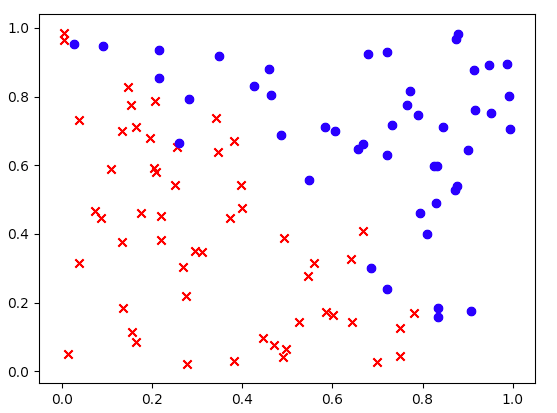
\includegraphics[width=\linewidth]{pics/F1b-b.png}
    \caption{Dataset A}\label{fig:dataset-a}
\end{subfigure}
\begin{subfigure}[b]{0.5\linewidth}
    \centering
    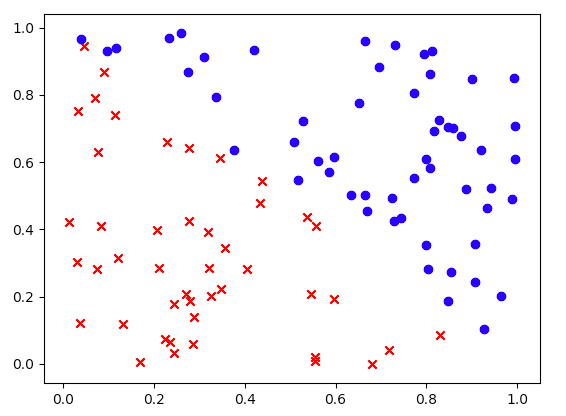
\includegraphics[width=\linewidth]{pics/F1b-a.png}
    \caption{Dataset B}\label{fig:dataset-b}
\end{subfigure}
\caption{Datasets}
\label{fig:datasets}
\end{figure}

Figure~\subref{fig:dataset-a} and Figure~\subref{fig:dataset-b} shows the two datasets. The problem is that dataset B is perfectly linearly separable. 

Consider optimizing objective:

$$
    L(\theta) = \prod_{i=1}^mp(y^{(i)}|x^{(i)};\theta) = \frac{1}{1 + e^{-y^{(i)}\theta^T x^{(i)}}}
$$

    Since the algorithm tries to find the maximum likelihood. if the data is linearly separable(i.e. all $y^{(i)}\theta^T x^{(i)}$ can be positive), every $ \frac{1}{1 + e^{-y^{(i)}\theta^T x^{(i)}}} $ can be small by augmenting the norm of $ \theta $ so after perfectly separate them the algorithm tends to augment $ \theta $ to infinity.
    
    If the data isn't linearly separable(i.e.  $\exists\  y^{(i)}\theta^T x^{(i)}$ to be negative), in this case, the algorithm cannot augment $ \theta $ infinitely since the negative $y^{(i)}\theta^T x^{(i)}$ constraints $ \frac{1}{1 + e^{-y^{(i)}\theta^T x^{(i)}}} $  to be very small while $ \|\theta\| $ is large. just like the regularization term. So there is a trade-off while maximizing the likelihood. 
\end{answer}


} \fi


  \item \subquestionpoints{5}
For each of these possible modifications, state whether or not it would lead to
the provided training algorithm converging on datasets such as $B$. Justify your
answers.
\begin{enumerate}
  \item Using a different constant learning rate.
  \item Decreasing the learning rate over time (e.g. scaling the initial
  learning rate by $1/t^2$, where $t$ is the number of gradient descent
  iterations thus far).
  \item Linear scaling of the input features.
  \item Adding a regularization term $\|\theta\|_2^2$ to the loss function.
  \item Adding zero-mean Gaussian noise to the training data or labels.
\end{enumerate}
 
\ifnum\solutions=1 {
  \begin{answer}
\begin{enumerate}
    \item No. $L(\theta)$ can still be arbitrarily large.
  \item Yes. When the learning rate is sufficiently small, the update to $\theta$ will be small, and it will be judged to be converged by the algorithm.
  \item No. The dataset will still be linearly seperable.
  \item Yes. In this case, scaling $\theta$ will not make the objective arbitrarily large.
  \item Yes. This will very likely make the dataset not linearly seperable.
  \item Yes. This will make the dataset not linearly separable, and easier to approach the global minimum.
\end{enumerate}

\end{answer}

} \fi

 
  
  \item \subquestionpoints{2}
Support vector machines (SVMs) are an alternative machine learning model that we discussed in class.
We have provided you an SVM implementation (using a radial basis function (RBF) kernel) within \texttt{src/svm.py} (You should not need to modify that code).

One important part of training an SVM parameterized by an RBF kernel is choosing an appropriate kernel radius.

Complete the \texttt{compute\_best\_svm\_radius} by writing code to compute the best SVM radius which maximizes accuracy on the validation dataset.

The provided code will use your \texttt{compute\_best\_svm\_radius} to compute and then write the best radius into \texttt{output/p06\_optimal\_radius}.

\ifnum\solutions=1 {
  \begin{answer}
    0.1 works best. The accuracy is 0.9695340501792115.
\end{answer}

} \fi



\end{enumerate}

\textbf{Hint:} Recall the distinction between functional margin and geometric
margin.

		
		\clearpage
\item \points{15} {\bf Logistic Regression: Training stability}

In this problem, we will be delving deeper into the workings of logistic
regression. The goal of this problem is to help you develop your skills
debugging machine learning algorithms (which can be very different from
debugging software in general).

We have provided a implementation of logistic regression in
\texttt{src/p01\_lr.py}, and two labeled datasets $A$ and $B$ in
\texttt{data/ds1\_a.txt} and \texttt{data/ds1\_b.txt}

Please do not modify the code for the logistic regression training algorithm
for this problem. First, run the given logistic regression code to train two
different models on $A$ and $B$. You can run the code by simply executing 
\texttt{python p01\_lr.py} in the \texttt{src} directory.

\begin{enumerate}

  \item \subquestionpoints{2}
What is the most notable difference in training the logistic regression model
on datasets $A$ and $B$?

\ifnum\solutions=1 {
  \begin{answer}
    Training on dataset A finished with few iterations, while with B it seems like a dead loop.
    
    P.S. I think the line \texttt{probs = 1. / (1 + np.exp(margins))} in the \texttt{cal\_grad} function of \texttt{src/p01\_lr.py} cannot be seen as probability (of a conventional Bernoulli distribution) because it is just a metric of margin.
    
    In fact if we choose $ \{0,1\} $ to represent label, we can write down the binary Bernoulli distribution $ B(\phi) $ and using GLM method to computer the expression of $ \phi $ as $ \frac{1}{1+\exp{-\theta^Tx}} $ so that this can be regarded as probability of being 1 given sample x.
    
    But that line only measure the margin between the point and the decision boundary. It cannot represent the probability of a point being classified as positive. 
    
\end{answer}

} \fi


  \item \subquestionpoints{5}
Investigate why the training procedure behaves unexpectedly on dataset $B$, but
not on $A$. Provide hard evidence (in the form of math, code, plots, etc.) to
corroborate your hypothesis for the misbehavior. Remember, you should address
why your explanation does \emph{not} apply to $A$.

\textbf{Hint}: The issue is not a numerical rounding or over/underflow error.

\ifnum\solutions=1 {
  
\begin{answer}

\begin{figure}[htbp]
\begin{subfigure}[b]{0.5\linewidth}
    \centering
    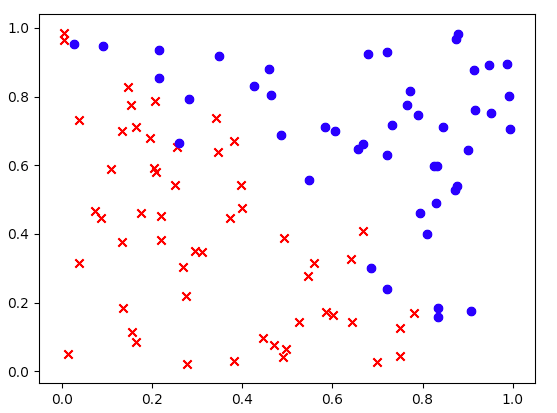
\includegraphics[width=\linewidth]{pics/F1b-b.png}
    \caption{Dataset A}\label{fig:dataset-a}
\end{subfigure}
\begin{subfigure}[b]{0.5\linewidth}
    \centering
    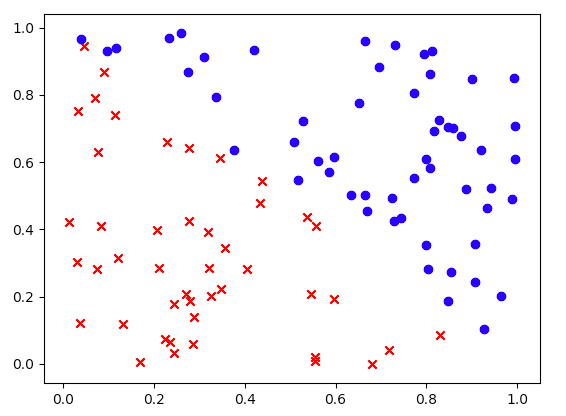
\includegraphics[width=\linewidth]{pics/F1b-a.png}
    \caption{Dataset B}\label{fig:dataset-b}
\end{subfigure}
\caption{Datasets}
\label{fig:datasets}
\end{figure}

Figure~\subref{fig:dataset-a} and Figure~\subref{fig:dataset-b} shows the two datasets. The problem is that dataset B is perfectly linearly separable. 

Consider optimizing objective:

$$
    L(\theta) = \prod_{i=1}^mp(y^{(i)}|x^{(i)};\theta) = \frac{1}{1 + e^{-y^{(i)}\theta^T x^{(i)}}}
$$

    Since the algorithm tries to find the maximum likelihood. if the data is linearly separable(i.e. all $y^{(i)}\theta^T x^{(i)}$ can be positive), every $ \frac{1}{1 + e^{-y^{(i)}\theta^T x^{(i)}}} $ can be small by augmenting the norm of $ \theta $ so after perfectly separate them the algorithm tends to augment $ \theta $ to infinity.
    
    If the data isn't linearly separable(i.e.  $\exists\  y^{(i)}\theta^T x^{(i)}$ to be negative), in this case, the algorithm cannot augment $ \theta $ infinitely since the negative $y^{(i)}\theta^T x^{(i)}$ constraints $ \frac{1}{1 + e^{-y^{(i)}\theta^T x^{(i)}}} $  to be very small while $ \|\theta\| $ is large. just like the regularization term. So there is a trade-off while maximizing the likelihood. 
\end{answer}


} \fi


  \item \subquestionpoints{5}
For each of these possible modifications, state whether or not it would lead to
the provided training algorithm converging on datasets such as $B$. Justify your
answers.
\begin{enumerate}
  \item Using a different constant learning rate.
  \item Decreasing the learning rate over time (e.g. scaling the initial
  learning rate by $1/t^2$, where $t$ is the number of gradient descent
  iterations thus far).
  \item Linear scaling of the input features.
  \item Adding a regularization term $\|\theta\|_2^2$ to the loss function.
  \item Adding zero-mean Gaussian noise to the training data or labels.
\end{enumerate}
 
\ifnum\solutions=1 {
  \begin{answer}
\begin{enumerate}
    \item No. $L(\theta)$ can still be arbitrarily large.
  \item Yes. When the learning rate is sufficiently small, the update to $\theta$ will be small, and it will be judged to be converged by the algorithm.
  \item No. The dataset will still be linearly seperable.
  \item Yes. In this case, scaling $\theta$ will not make the objective arbitrarily large.
  \item Yes. This will very likely make the dataset not linearly seperable.
  \item Yes. This will make the dataset not linearly separable, and easier to approach the global minimum.
\end{enumerate}

\end{answer}

} \fi

 
  
  \item \subquestionpoints{2}
Support vector machines (SVMs) are an alternative machine learning model that we discussed in class.
We have provided you an SVM implementation (using a radial basis function (RBF) kernel) within \texttt{src/svm.py} (You should not need to modify that code).

One important part of training an SVM parameterized by an RBF kernel is choosing an appropriate kernel radius.

Complete the \texttt{compute\_best\_svm\_radius} by writing code to compute the best SVM radius which maximizes accuracy on the validation dataset.

The provided code will use your \texttt{compute\_best\_svm\_radius} to compute and then write the best radius into \texttt{output/p06\_optimal\_radius}.

\ifnum\solutions=1 {
  \begin{answer}
    0.1 works best. The accuracy is 0.9695340501792115.
\end{answer}

} \fi



\end{enumerate}

\textbf{Hint:} Recall the distinction between functional margin and geometric
margin.

		
	\end{enumerate}
	
\end{document}
